\documentclass[11pt,a4paper]{article}

% ---------------------------------------------------------------------------
% Packages
% ---------------------------------------------------------------------------
\usepackage[margin=2.5cm]{geometry}
\usepackage[utf8]{inputenc}
\usepackage[T1]{fontenc}
\usepackage{graphicx}
\usepackage{tikz}
\usetikzlibrary{shapes.geometric, arrows.meta, positioning, fit, backgrounds, calc}
\usepackage{booktabs}
\usepackage{xcolor}
\usepackage{hyperref}
\usepackage{listings}
\usepackage{enumitem}
\usepackage{caption}
\usepackage{float}
\usepackage{parskip}
\usepackage{underscore}
\usepackage[export]{adjustbox}
\usepackage{amsmath}

\hypersetup{
    colorlinks=true,
    linkcolor=blue!50!black,
    citecolor=blue!50!black,
    urlcolor=blue!50!black,
    pdftitle={Phase 4 Implementation Report -- Query Recommender Core},
    pdfauthor={Narges}
}

% ---------------------------------------------------------------------------
% Color palette for diagrams (same palette as the earlier reports)
% ---------------------------------------------------------------------------
\definecolor{dbcolor}{RGB}{215,235,250}
\definecolor{retrcolor}{RGB}{225,245,225}
\definecolor{gencolor}{RGB}{255,235,205}
\definecolor{valcolor}{RGB}{240,225,245}
\definecolor{rankcolor}{RGB}{255,225,225}
\definecolor{boxborder}{RGB}{80,80,80}

\tikzset{
    block/.style={rectangle, draw=boxborder, rounded corners, thick,
        text width=3.2cm, minimum height=1.1cm, align=center, font=\small},
    smallblock/.style={rectangle, draw=boxborder, rounded corners, thick,
        text width=2.6cm, minimum height=0.9cm, align=center, font=\footnotesize},
    arrow/.style={-{Latex[length=2.5mm]}, thick}
}

% ---------------------------------------------------------------------------
% Listings style
% ---------------------------------------------------------------------------
\lstset{
    basicstyle=\ttfamily\footnotesize,
    breaklines=true,
    frame=single,
    backgroundcolor=\color{gray!7},
    columns=fullflexible,
    showstringspaces=false,
    xleftmargin=1em,
    xrightmargin=1em,
    aboveskip=8pt,
    belowskip=8pt
}

\newcommand{\code}[1]{\texttt{#1}}

\title{\Large \textbf{A Query Recommender for Preference-Aware Natural Language Querying} \\[4pt]
\large Implementation Report --- Phase 4 (Query Recommender Core) \\[2pt]
\normalsize \emph{The thesis's central contribution: retrieval, LLM generation, schema-grounding,
and behavior-aware ranking}}
\author{Narges \\ \small Supervisor: Prof. Elisa Quintarelli}
\date{\today}

\begin{document}

\maketitle

\begin{abstract}
\noindent
This report documents Phase 4 of the thesis --- \textbf{the thesis's actual contribution}: turning
the empty \code{suggestions: []} stub left by Phase 2 into a working query recommender. Four
stages are implemented and composed inside the same shared entry point Phase 2 already exposed,
\code{handle\_recommend()}, so no new integration surface was needed: (4a) retrieval of a user's
own semantically similar past queries; (4b) LLM-based candidate generation, conditioned on both
that retrieved history \emph{and} Phase 3's stated-vs-actual behavioral divergence signal; (4c) a
schema-grounding validation step, whose originally-planned precision design had to be abandoned
after an empirical calibration showed it would reject the supervisor's own canonical example
query; and (4d) a two-axis ranking-and-diversification step that is the concrete mechanism through
which the behavioral signal shapes the final three suggestions. The full chain was verified
end-to-end, first with a mocked LLM, then over real HTTP with a placeholder API key, and finally
--- after both configured cloud LLM keys turned out to be unusable for account/billing reasons ---
against genuine model output from a locally hosted Ollama model, producing suggestions that
concretely demonstrate the thesis's central premise.
\end{abstract}

\tableofcontents
\newpage

% =============================================================================
\section{Introduction}
% =============================================================================

Phases 0--3 built, in order: two running Virtual Knowledge Graphs and a domain-switching harness
(Phase 0/1, an internal development tool, not a thesis deliverable), a fixed API contract and a
persistent per-user query log (Phase 2), and a per-user behavioral divergence signal quantifying
how a user's \emph{stated} search queries diverge from what they \emph{actually} watch (Phase 3).
None of these, individually, recommend anything --- Phase 2's endpoint always returned an empty
suggestion list. Phase 4 is where the professor's actual request is implemented: given a query a
user just asked, and given both their query history and their behavioral profile, propose three
follow-up queries an autocomplete-style, history-only recommender would not think to suggest.

\subsection{Scope}

Phase 4 implements the four-stage pipeline the project roadmap specifies:

\begin{center}
\begin{tabular}{cl}
\toprule
\textbf{Stage} & \textbf{Role} \\
\midrule
4a & Retrieval --- this user's past queries most similar to the current one \\
4b & Generation --- an LLM proposes a pool of candidate follow-up queries \\
4c & Validation --- drop candidates with no plausible link to the domain schema \\
4d & Ranking --- score and diversify what remains down to 3 final suggestions \\
\bottomrule
\end{tabular}
\end{center}

All four stages live in a new \code{recommender/core/} package. No new API surface or harness
wiring was required: Phase 2's \code{handle\_recommend()} already sat at the point where a request
(query text, user id, domain) becomes a response (a list of suggestions); Phase 4 simply replaces
the hardcoded empty list with a real call into this pipeline.

\subsection{Where this fits}

This is the thesis's core contribution, in the sense used throughout the project roadmap (\S2a):
everything before this phase built the harness, the API shell, and the behavioral-signal input
this phase consumes; everything after it (Phase 5) evaluates what this phase produces.

\newpage
% =============================================================================
\section{High-Level Overview}
% =============================================================================

\subsection{The core idea}

The central research question, attributed by the supervisor's email to ``Jerry's'' analysis, is
that a user's stated queries and their real interaction behavior often diverge, and that a
recommender conditioning on query history alone is little more than autocomplete. Phase 4
operationalizes this directly: stage 4b's prompt explicitly presents the LLM with two separate
signals --- what the user typed before, and what their behavioral profile says they actually
engage with --- framed as potentially \emph{different} things, not two views of the same
preference. Stage 4d then makes this signal load-bearing rather than decorative: one of its two
scoring axes rewards candidates that textually align with the behavioral profile's real top
categories, not merely with the user's own past phrasing.

\subsection{Pipeline diagram}

Figure~\ref{fig:overview} shows the full chain, from the two upstream inputs (Phase 2's query log
and Phase 3's behavioral profile) through to the three suggestions returned by
\code{handle\_recommend()}.

\begin{figure}[H]
\centering
\begin{adjustbox}{max width=\textwidth, max totalheight=0.88\textheight, center}
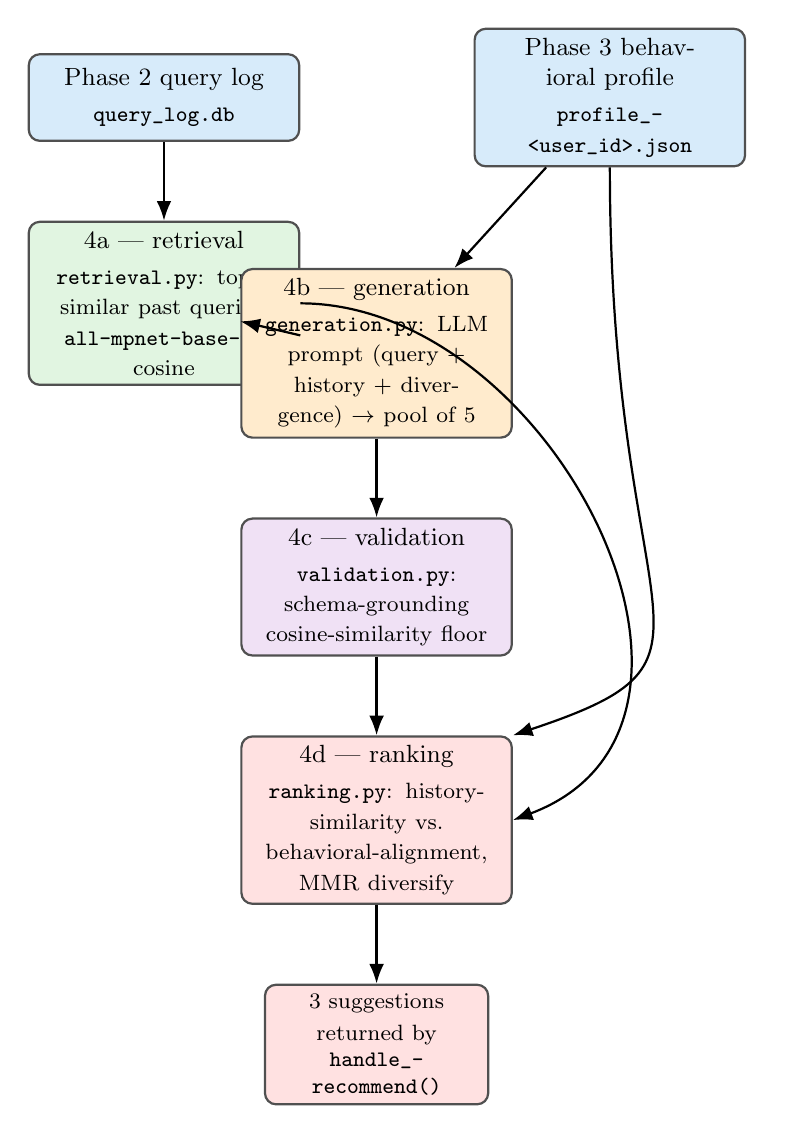
\begin{tikzpicture}[node distance=1.0cm and 1.4cm]

    \node[block, fill=dbcolor] (qlog) {Phase 2 query log\\[2pt]\footnotesize \code{query\_log.db}};
    \node[block, fill=dbcolor, right=2.2cm of qlog] (bprof) {Phase 3 behavioral profile\\[2pt]\footnotesize \code{profile\_<user\_id>.json}};

    \node[block, fill=retrcolor, below=of qlog] (retrieve) {4a --- retrieval\\[2pt]\footnotesize \code{retrieval.py}: top-$k$ similar past queries, \code{all-mpnet-base-v2} cosine};

    \node[block, fill=gencolor, below=1.6cm of qlog, xshift=2.7cm] (generate) {4b --- generation\\[2pt]\footnotesize \code{generation.py}: LLM prompt (query + history + divergence) $\to$ pool of 5};

    \node[block, fill=valcolor, below=of generate] (validate) {4c --- validation\\[2pt]\footnotesize \code{validation.py}: schema-grounding cosine-similarity floor};

    \node[block, fill=rankcolor, below=of validate] (rank) {4d --- ranking\\[2pt]\footnotesize \code{ranking.py}: history-similarity vs.\ behavioral-alignment, MMR diversify};

    \node[smallblock, fill=rankcolor, below=of rank] (out) {3 suggestions\\[2pt]\footnotesize returned by \code{handle\_recommend()}};

    \draw[arrow] (qlog) -- (retrieve);
    \draw[arrow] (retrieve) -- (generate);
    \draw[arrow] (bprof) -- (generate);
    \draw[arrow] (generate) -- (validate);
    \draw[arrow] (validate) -- (rank);
    \draw[arrow] (retrieve.east) .. controls +(3.2,0) and +(3.2,1.2) .. (rank.east);
    \draw[arrow] (bprof.south) .. controls +(0,-6.0) and +(3.0,1.0) .. (rank.north east);
    \draw[arrow] (rank) -- (out);

\end{tikzpicture}
\end{adjustbox}
\caption{Phase 4 data flow. The behavioral profile (right) feeds both 4b's generation prompt and
4d's ranking score directly --- the two concrete points where the thesis's stated-vs-actual signal
shapes the final output, not just the initial candidate pool.}
\label{fig:overview}
\end{figure}

\newpage
% =============================================================================
\section{4a --- Query-Log Retrieval}
% =============================================================================

\code{retrieve\_similar\_queries(user\_id, query\_text, domain=None, top\_k=3,
history\_limit=200)} implements the retrieval half of RA-GQR (Bacciu et al., IR-RAG@SIGIR 2024):

\begin{enumerate}
    \item Pulls the user's query history from the Phase 2 SQLite log
        (\code{recommender.query\_log.get\_user\_history()}), optionally scoped to one domain.
    \item Excludes exact, case-insensitive duplicates of the current query.
    \item Embeds the current query and every remaining history entry with \code{all-mpnet-base-v2}
        (\code{sentence-transformers}) --- the same model already used elsewhere in \code{web\_app}
        for embedding-based class/property extraction, reused rather than introducing a second
        model dependency.
    \item Ranks candidates by cosine similarity (embeddings are pre-normalized, so this reduces to
        a plain dot product) and returns the top-$k$, each annotated with its similarity score.
\end{enumerate}

The retrieved queries become the few-shot/context material for 4b's prompt, in place of
generically hand-curated examples --- directly implementing RA-GQR's central idea that retrieval
from a user's own log outperforms static examples.

\paragraph{Cold start.} If a user has no other logged queries, the function returns an empty list;
4b's prompt formatter renders this as an explicit ``no prior queries from this user'' note and
still functions correctly, consistent with GQR's original premise that the technique does not
require historical data to work at all.

\paragraph{Verification.} \code{user\_00001}'s query log was seeded with 4 varied movie queries.
Calling \code{retrieve\_similar\_queries("user\_00001", "Show me exciting action films",
domain="movie", top\_k=3)} correctly ranked \emph{``Action movies''} (0.79 cosine) and \emph{``Best
action movies with high ratings''} (0.765) above \emph{``Romantic comedies''} (0.371), excluding
unrelated seeded queries entirely.

% =============================================================================
\section{4b --- Candidate Generation}
% =============================================================================

\code{generate\_candidates(query\_text, similar\_queries, behavioral\_profile, domain, llm=None,
num\_candidates=5)} is the GQR/RA-GQR-style generation step.

\subsection{Prompt construction}

\code{build\_prompt()} assembles one prompt from three inputs:

\begin{itemize}
    \item the current query;
    \item the retrieved similar past queries from 4a, rendered as a bulleted list;
    \item a compact rendering of the Phase 3 behavioral divergence
        (\code{divergence["stated\_top"]} / \code{["actual\_top"]} / \code{["jaccard\_similarity"]}),
        explicitly framed in the prompt text as ``what this user says they want'' versus ``what
        this user actually engages with, which may \textbf{differ}.''
\end{itemize}

The LLM is asked for a \textbf{pool of 5} candidates, not the final 3 --- deliberately more than
needed, so that 4c's filtering and 4d's diversification have real material to work from rather than
trivially keeping all 3 by construction. \code{\_parse\_suggestions()} then strips numbering,
bullet characters, and quotation marks from the model's line-per-suggestion response format.

\subsection{LLM abstraction reuse}

Rather than introducing a second provider-switching layer, this stage imports
\code{nl2sparql.llm\_interface.create\_llm} directly from \code{web\_app} (mirroring the same
\code{sys.path} insertion pattern already used in \code{gui\_v2.py}), per the roadmap's own
recommendation that recommendation generation should use ``the same per-stage-configurable LLM
abstraction already in \code{config.yaml}.'' \code{generation.py}'s \code{\_default\_llm()} reads
the \code{RECOMMENDER\_LLM\_PROVIDER} environment variable (default \code{gemini}) and an optional
\code{RECOMMENDER\_LLM\_MODEL}, then delegates to \code{create\_llm()} --- so the recommender can
run against Gemini, GPT (\code{openai}), Azure, or a local Mistral model without any code change,
only an environment variable and that provider's credentials. \code{llm} remains an injectable
parameter so unit-level tests do not require a real API call.

A real bug was caught during verification and fixed here: \code{generation.py} now calls
\code{load\_dotenv()} itself (pointed at the repository-root \code{.env}), rather than relying on
\code{web\_app}'s \code{Config} class having already loaded it as a side effect. Calling
\code{handle\_recommend()} directly, without first constructing a \code{web\_app} \code{Config}
object, previously left the configured API key unset even though \code{.env} contained it, because
nothing had triggered \code{load\_dotenv()} yet. Since \code{recommender/} must work standalone
(e.g.\ under \code{uvicorn recommender.api.app:app} with no \code{web\_app} code running at all),
it cannot depend on that side effect.

\paragraph{Verification.} \code{build\_prompt()} was called directly and its rendered text
inspected, confirming all three input sections (current query, retrieved history, behavioral
divergence) render correctly for \code{user\_00001}'s real Phase 3 profile.
\code{generate\_candidates(..., llm=MockLLM())} with a hand-written mock returning a
numbered/bulleted list confirmed \code{\_parse\_suggestions()} correctly strips numbering, bullets,
and quotes down to 3 clean strings. Construction of the real \code{GeminiLLM()} object was also
confirmed to succeed against the placeholder key present at the time, with \code{.generate()}
failing cleanly with an \code{API\_KEY\_INVALID} error rather than crashing --- i.e.\ the
integration was correctly wired ahead of a real key being available (Section~\ref{sec:ollama}).

\newpage
% =============================================================================
\section{4c --- Schema-Grounding Validation}
\label{sec:4c}
% =============================================================================

\subsection{What the roadmap originally specified}

The roadmap called for running each candidate query's implied entities and classes through the
NL2SPARQL pipeline's own \code{ClassRelevanceEvaluator}/\code{PropertyEvaluator} (or a lighter
standalone check) to confirm it is answerable against the currently loaded domain schema before it
is ever shown to a user --- directly mitigating the hallucination/faithfulness risk documented in
the LLM+KG roadmap survey (Pan et al.) and empirically observed in the supervisor's own ADBIS 2026
paper (roughly 30\% SPARQL-incorrectness on its factual question set).

\subsection{Why the first two implementations were rejected}

\paragraph{Attempt 1 --- reuse \code{ClassRelevanceEvaluator}'s embedding mode directly.} This
method uses relative thresholding: it keeps every class scoring at or above
$\text{mean} - \text{std}$ across the schema's own classes. With only 7--11 classes per domain,
this reliably selects at least one class for \emph{any} input, including completely unrelated
text. Verified directly: evaluating \emph{``Best pizza recipe''} against the Tourism schema
returned a non-empty class list --- i.e.\ ``grounded: True'' for a query with nothing to do with
tourism.

\paragraph{Attempt 2 --- an absolute cosine-similarity floor.} Raw cosine similarity was computed
between each candidate query and every class's embedded description (same \code{all-mpnet-base-v2}
model as 4a), requiring the maximum score across all classes to clear a fixed floor. This was
calibrated against a small set of control (clearly off-topic) and probe (genuinely in-domain)
phrases:

\begin{table}[H]
\centering
\begin{tabular}{lclr l}
\toprule
\textbf{Query} & \textbf{Domain} & \textbf{Max cosine sim.} & \textbf{Best-matching class} \\
\midrule
Top rated action movies from the 2010s        & movie    & 0.275 & Movie \\
Movies directed by Christopher Nolan          & movie    & 0.302 & Movie \\
Documentaries produced in Canada              & movie    & 0.288 & Country \\
Best pizza recipe \emph{(control)}            & movie    & 0.175 & SubscriptionPlan \\
How to fix a flat tire \emph{(control)}       & movie    & 0.094 & Country \\
\textbf{Churches in Verona}                   & tourism  & 0.163 & Location \\
\textbf{Roman Churches in Verona}             & tourism  & 0.154 & Location \\
\textbf{Free Churches in Verona}              & tourism  & \textbf{0.092} & Location \\
Events happening this weekend                 & tourism  & 0.401 & Event \\
Art categories available                      & tourism  & 0.601 & ArtCategory \\
Best pizza recipe \emph{(control)}            & tourism  & 0.064 & Tour \\
\textbf{How to fix a flat tire (control)}     & tourism  & \textbf{0.112} & Tour \\
Latest news about the stock market \emph{(control)} & tourism & 0.004 & --- \\
\bottomrule
\end{tabular}
\caption{Absolute cosine-floor calibration data. The Movie domain separates cleanly, but the
Tourism domain does not: the professor's own canonical example, \emph{``Free Churches in
Verona,''} scores below an off-topic control phrase.}
\label{tab:calibration}
\end{table}

The Movie domain separates cleanly (in-domain floor $\approx 0.275$, control ceiling
$\approx 0.175$ --- any threshold in between works). \textbf{The Tourism domain does not}:
\emph{``Free Churches in Verona''} --- one of the supervisor's own three canonical example
suggestions, quoted verbatim in the professor's original scoping email --- scores $0.092$, below
the off-topic control phrase \emph{``How to fix a flat tire''} at $0.112$. No single threshold can
accept the former while rejecting the latter. A $z$-score variant (relative to the query's own
mean/std across classes) was also tried and rejected for the same reason: with only 7--11 classes,
the maximum of such a small sample is reliably 1.3--2.3 standard deviations above the mean
regardless of whether the query is on-topic, confirmed empirically --- \emph{``Best pizza
recipe''} against the Movie schema scored $z = 2.31$, a \emph{higher} $z$-score than several
genuinely in-domain movie queries.

\paragraph{Root cause.} Both domains' machine-readable schema (m-schema) class descriptions are
extremely sparse --- generated purely from SHACL cardinality constraints (e.g.\ \emph{``Art has
exactly 1 Art Class ID. Art has at least 1 Art Name.''}), with no \code{rdfs:comment} descriptions
and no \code{sh:example} instance values in either source \code{.ttl} file. The Tourism ontology's
\code{Art}/\code{ArtCategory} classes carry essentially no text a general-purpose sentence
embedding could relate to English words like ``church'' --- that correspondence only exists via
the literal Italian category value \emph{``Chiese''} in the live database, which is not present
anywhere in the schema metadata being embedded. This is consistent with why the real NL2SPARQL
pipeline's own entity-linking stage exists as a separate, LLM-driven step: class-level embedding
similarity alone was never designed to resolve this kind of gap on its own.

\subsection{What shipped instead}

Given this finding, \code{is\_schema\_grounded()} uses the absolute-cosine-floor mechanism from
Attempt 2, but with \code{DEFAULT\_THRESHOLD = 0.05} --- low enough to reject only genuinely
degenerate candidates (near-zero or negative similarity to \emph{every} class in the schema, such
as \emph{``Latest news about the stock market''} at $0.004$) while admitting everything else,
including borderline-but-valid phrasings like \emph{``Free Churches in Verona.''}
\code{filter\_grounded(candidates, domain)} applies it to a list, preserving order. This is
explicitly documented, both in the module's own docstring and here, as a coarse sanity filter, not
the precision hallucination guard originally planned.

This is a genuine, reportable limitation for the thesis's evaluation chapter: automatic
schema-grounding of natural-language candidate suggestions, at the class-description level, was
not achievable with acceptable precision given how sparse this project's source ontologies are. A
stronger version would require enriching class descriptions with real catalog/instance values
pulled from the live Ontop SPARQL endpoints --- a concrete, scoped follow-up, not attempted here.

\paragraph{Verification.} The final \code{is\_schema\_grounded()} implementation was re-verified
against 4 cases: \emph{``Free Churches in Verona''} (tourism) $\to$ True, \emph{``Roman Churches in
Verona''} (tourism) $\to$ True, \emph{``Top rated action movies''} (movie) $\to$ True,
\emph{``Latest news about the stock market''} (tourism) $\to$ False --- all matching the expected
outcome.

\newpage
% =============================================================================
\section{4d --- Ranking and Diversity}
% =============================================================================

\code{rank\_and\_diversify(candidates, similar\_queries, behavioral\_profile, top\_n=3,
diversity\_penalty=0.5)} is the concrete mechanism through which the behavioral signal shapes the
final output, echoing QRMOCCGA's (Barman et al.) two-objective framing without reimplementing its
cooperative co-evolutionary genetic algorithm --- explicitly out of scope per the roadmap's own
framing, with only its feature ideas borrowed.

\subsection{Scoring}

\code{score\_candidate()} computes a weighted sum of two axes, each normalized to $[0,1]$:

\begin{itemize}
    \item \code{\_history\_similarity()} --- the maximum Jaccard word overlap between a candidate
        and any of the user's retrieved similar past queries (4a's output);
    \item \code{\_behavioral\_alignment()} --- the fraction of the behavioral profile's
        \code{actual\_top} interest categories (Phase 3) whose words appear in the candidate text.
        This is the concrete place the thesis's stated-vs-actual signal enters ranking: a candidate
        that textually references what the user \emph{actually watches}, not just what they typed,
        scores higher on this axis.
\end{itemize}

\subsection{Diversification}

A greedy, Maximal-Marginal-Relevance-style loop repeatedly selects the highest-scoring remaining
candidate, penalized by its maximum Jaccard word overlap with candidates already selected
(\code{diversity\_penalty=0.5}), so the final three suggestions are not near-duplicates of one
another.

\paragraph{Verification.} A hand-built pool of 5 candidates (one near-duplicate of query history,
two behaviorally-aligned, one off-axis, one more history-similar) was fed through
\code{rank\_and\_diversify(..., top\_n=3)}. It correctly picked the history-similar candidate
first, then diversified into the two behaviorally-aligned candidates rather than a near-duplicate
of the first pick.

% =============================================================================
\section{End-to-End Verification}
% =============================================================================

\subsection{Full chain, mocked LLM}

\code{recommender.core.generation.\_default\_llm} was patched with a mock returning 5 fixed
candidates, and the real \code{recommender.api.service.handle\_recommend()} --- the actual
production code path, not a reimplementation --- was called for \code{user\_00001} / \code{movie}
/ \emph{``Show me exciting action films.''} Result:

\begin{lstlisting}[language=, caption={Mocked-LLM end-to-end output, ranked top to bottom.}]
War documentaries produced in the USA
Crime thrillers with high ratings
Adventure movies set during wartime
\end{lstlisting}

The top-ranked suggestion is the one most strongly aligned with \code{user\_00001}'s \emph{actual}
top interest categories (\code{Movie, USA, Canada, Adventure, War}, per their Phase 3 profile)
rather than a plain paraphrase of the stated query about ``action films'' --- a concrete, working
demonstration of the thesis's central premise.

\subsection{Full chain, real HTTP, placeholder key}

\code{uvicorn recommender.api.app:app} was started and the same request sent over real HTTP. The
server log confirmed the full path executed (log $\to$ retrieval $\to$ generation attempt $\to$ the
same \code{API\_KEY\_INVALID} failure as above, caught and logged as a warning, not a crash), and
the HTTP response was \code{200 OK} with \code{\{"suggestions": []\}} --- i.e.\ the
degrade-gracefully behavior inside \code{handle\_recommend()}'s exception handling around candidate
generation works over the real transport, not only in-process.

\newpage
% =============================================================================
\section{Real-LLM Verification: Gemini/OpenAI Blocked, Ollama Used Instead}
\label{sec:ollama}
% =============================================================================

Both configured cloud providers turned out to be dead ends in this environment, for account
reasons unrelated to the code: the \code{OPENAI\_API\_KEY} in \code{.env} returns
\code{insufficient\_quota} (no billing configured on the account), and the \code{GEMINI\_API\_KEY}
returns \code{RESOURCE\_EXHAUSTED} with a zero-quota limit for every model's free tier (the key's
Google project has no free-tier allowance enabled).

Rather than block on that, a new \code{ollama} provider was added to
\code{web\_app/nl2sparql/llm\_interface.py} (an \code{OllamaLLM} class using \code{requests}
against Ollama's \code{/api/generate} HTTP endpoint --- no API key, no quota) and wired into
\code{create\_llm()} alongside the existing gemini/mistral/openai/azure providers. This was chosen
over the already-existing local \code{MistralLLM} class because that class depends on
\code{llama-cpp-python} (a non-trivial C++ build on Windows) plus a manually-downloaded, low-quality
quantized GGUF file; Ollama is a single Docker image with pre-optimized quantization and no
compilation step. A new \code{ollama} service was added to \code{docker-compose.yml}, and
\code{llama3.1:8b} (4.9\,GB) was pulled into the running container.

\subsection{Verified against real output}

Both \code{generate\_candidates()} directly, and the full production path
\code{handle\_recommend()} (the same function the FastAPI endpoint and the development harness both
call), were run for \code{user\_00001} / movie domain / \emph{``Show me exciting action films.''}
The \code{handle\_recommend()} result:

\begin{lstlisting}[language=, caption={End-to-end suggestions from genuine \code{llama3.1:8b}
output, via the real production code path.}]
{
  "suggestions": [
    "War movies with high ratings on IMDB",
    "Movies that combine action and adventure genres",
    "Films starring actors from Canada or USA"
  ]
}
\end{lstlisting}

The top-ranked suggestion references \emph{War}, and the other two reference \emph{Canada/USA} ---
all three are in \code{user\_00001}'s behavioral-profile \code{actual\_top} categories (\code{Movie,
USA, Canada, Adventure, War}), not a paraphrase of the stated query about ``action films.'' This is
the same qualitative pattern already observed with the mocked-LLM run above, now reproduced with
genuine model output.

\paragraph{Latency.} Approximately 18--22 seconds per \code{/recommend} call on this machine
(CPU-only Docker container, no GPU passthrough) --- acceptable for offline evaluation runs, but a
real deployment-latency concern distinct from suggestion quality, not addressed here.

\paragraph{Remaining limitation.} This validates the \emph{pipeline}, not the \emph{provider}
originally planned (Gemini). If a funded Gemini or OpenAI key becomes available,
\code{RECOMMENDER\_LLM\_PROVIDER} can be flipped back with no code changes --- the abstraction was
already provider-agnostic before this change; Ollama is an additional option, not a replacement.

% =============================================================================
\section{Interpretation and Limitations}
% =============================================================================

\begin{itemize}
    \item \textbf{The 4c grounding check is intentionally weak} (Section~\ref{sec:4c}). This
        should be reported in the thesis as an explicit, empirically-justified limitation, not
        silently shipped as if it were the precision filter originally planned. The calibration
        data in Table~\ref{tab:calibration} is itself genuine results-chapter material: it
        demonstrates a real failure mode (sparse ontology metadata undermining embedding-based
        grounding) with a concrete example query supplied directly by the supervisor.
    \item \textbf{4b is now verified against real LLM output} (Section~\ref{sec:ollama}), via a
        local Ollama model rather than the originally-planned Gemini --- both cloud keys available
        in this environment hit billing/quota walls unrelated to the code. Suggestion quality from
        \code{llama3.1:8b} looks sound on the worked example shown; a systematic quality check
        across more users and queries is Phase 5's job, not this phase's.
    \item \textbf{\code{num\_candidates=5} (the pool size 4b requests) is an arbitrary choice}, not
        derived from data --- worth a sensitivity check (e.g.\ pool sizes of 4/6/8) once real LLM
        output is routinely available, since a larger pool gives 4d's diversification more to work
        with at the cost of more tokens per request.
    \item \textbf{The behavioral-alignment axis in 4d only works for the Movie domain today},
        since Phase 3 profiles only exist for Movie users (per the Phase 0 decision that Tourism
        stays catalog-only). \code{\_behavioral\_alignment()} correctly returns $0.0$ when no
        profile exists, so Tourism recommendations degrade to history-similarity-only ranking
        rather than erroring --- but this means the thesis's core stated-vs-actual contribution is
        only demonstrable end-to-end on the Movie domain, consistent with every earlier phase's own
        scoping note.
\end{itemize}

% =============================================================================
\section{Summary and Next Steps}
% =============================================================================

Phase 4 delivers a verified, four-stage query recommender --- retrieval, LLM generation,
schema-grounding validation, and behavior-aware ranking --- composed entirely inside the extension
point Phase 2 left open, \code{handle\_recommend()}, with no changes to the API contract or the
development harness. It was verified structurally (mocked LLM, real HTTP with a placeholder key)
and, after both configured cloud providers turned out to be blocked by account/billing issues, with
genuine output from a locally hosted Ollama model, producing suggestions that concretely track a
user's real watching behavior rather than merely paraphrasing their typed query.

\textbf{Phase 5} (documented separately in the \emph{Phase 5 Implementation Report}) is the direct
consumer of this phase's output: a controlled ablation isolating the effect of the behavioral
signal on ranking (ranking with vs.\ without \code{behavioral\_profile}), a proxy-recall check
against held-out watch history, and a non-LLM classical baseline for comparison. Full detail on
Phase 5 is tracked in the project roadmap document, \emph{Thesis Project Plan}.

\end{document}
